% =============================================================================
%  General Response Template — Reviewer Comments
%  Paper: Explainable AI for Student Success: A Multi-Objective Framework with
%         SHAP-Based Personalized Recommendations
%  Authors: Shikha Pachouly, D. S. Bormane
%
%  Compile with pdflatex (no shell-escape needed).
%  This template is designed to be extended with additional reviewer comments
%  and responses as needed.
% =============================================================================

\documentclass[11pt,a4paper]{article}

% ---- Geometry & typography --------------------------------------------------
\usepackage[a4paper,margin=1in]{geometry}
\usepackage{lmodern}
\usepackage[T1]{fontenc}
\usepackage[utf8]{inputenc}
\usepackage{microtype}
\usepackage{setspace}
\onehalfspacing

% ---- Tables, math, lists ----------------------------------------------------
\usepackage{array}
\usepackage{booktabs}
\usepackage{tabularx}
\usepackage{longtable}
\usepackage{multirow}
\usepackage{amsmath,amssymb}
\usepackage{enumitem}
\usepackage{graphicx}
\setlist[itemize]{leftmargin=1.4em,topsep=2pt,itemsep=2pt}
\setlist[enumerate]{leftmargin=1.6em,topsep=2pt,itemsep=2pt}
\setlist[description]{leftmargin=0pt,topsep=2pt,itemsep=2pt}

% ---- Color & links ----------------------------------------------------------
\usepackage[dvipsnames]{xcolor}
\definecolor{revred}{HTML}{C00000}
\definecolor{accentblue}{HTML}{1F4E79}
\definecolor{lightgray}{HTML}{F2F2F2}
\usepackage[colorlinks=true,linkcolor=accentblue,urlcolor=accentblue,
            citecolor=accentblue,pdfborder={0 0 0}]{hyperref}

% Prevent hyphenation and ensure URLs break properly
\usepackage{url}
\urlstyle{same}
\hyphenpenalty=10000
\exhyphenpenalty=10000

% ---- Shaded boxes for reviewer quotes ---------------------------------------
\usepackage{tcolorbox}
\tcbuselibrary{breakable,skins}
\newtcolorbox{reviewerquote}[1][]{%
  enhanced,breakable,
  colback=lightgray,colframe=lightgray,
  boxrule=0pt,leftrule=2pt,
  leftrule=2pt,colframe=accentblue!70,
  arc=0pt,outer arc=0pt,
  left=10pt,right=10pt,top=4pt,bottom=4pt,
  fontupper=\itshape,
  before skip=4pt,after skip=4pt,
  #1
}
\newtcolorbox{evidencebox}[1][]{%
  enhanced,breakable,
  colback=accentblue!4,colframe=accentblue!50,
  boxrule=0.4pt,arc=2pt,
  left=8pt,right=8pt,top=4pt,bottom=4pt,
  before skip=4pt,after skip=4pt,
  #1
}
\newtcolorbox{correctionbox}[1][]{%
  enhanced,breakable,
  colback=revred!4,colframe=revred!50,
  boxrule=0.4pt,arc=2pt,
  left=8pt,right=8pt,top=4pt,bottom=4pt,
  before skip=4pt,after skip=4pt,
  #1
}

% ---- Comment-id badge (e.g., "R1.4")  --------------------------------------
\newcommand{\cid}[1]{\textcolor{revred}{\textbf{[#1]}}}
\newcommand{\filebox}[1]{\texttt{\small #1}}
\newcommand{\sectref}[1]{Section~#1}
\newcommand{\sectreflower}[1]{section~#1}
\newcommand{\stress}[1]{\textbf{#1}}

% ---- Header / Title ---------------------------------------------------------
\usepackage{fancyhdr}
\pagestyle{fancy}
\fancyhf{}
\fancyhead[L]{\small General Response to Reviewer Comments}
\fancyhead[R]{\small Page \thepage}
\renewcommand{\headrulewidth}{0.4pt}

% =============================================================================
\begin{document}

\begin{center}
  {\LARGE\bfseries  Response to Reviewer Comments}\\[6pt]
  {\large International Journal of Intelligent Engineering and Systems (IJIES)}\\[2pt]
  Paper ID \textbf{20262542}
\end{center}

\vspace{4pt}
\noindent\textbf{Title:}~Explainable AI for Student Success: A Multi-Objective Framework with SHAP-Based Personalized Recommendations.\\
\textbf{Authors:}~Shikha Pachouly, D. S. Bormane.\\

\textbf{Note:}~ All the Changes of Second Revision are highlighted with Yellow Hihglight and Red Font.

\vspace{6pt}
\hrule
\vspace{6pt}

% =============================================================================
% ADD NEW REVIEWER COMMENTS BELOW
% Use the following template for each new comment:
%
% \subsection*{\cid{[ID]}~~[Short Title]}
%
% \begin{reviewerquote}
% ``[Reviewer's exact comment]''
% \end{reviewerquote}
%
% \paragraph{Action.} [Description of action taken]
%
% \paragraph{Evidence.} [Supporting evidence, file references, corrected values, etc.]
%
% =============================================================================

% =============================================================================
% EXAMPLE: Numerical Correction (Already completed)
% =============================================================================

\subsection*{\cid{CORR-1}~~Table 2 Delta Calculation Error}

\begin{reviewerquote}
``In Table 2, the reported delta for the CGPA Category task is numerically inconsistent. The difference between 0.451 and 0.387 is 0.064, not 0.063. Please verify whether this is a rounding issue or a calculation error.''
\end{reviewerquote}

\paragraph{Verification.}
\[
0.451 - 0.387 = 0.064
\]

Please Note The table referred in observation 1 is Table 3 not Table 2 so I have Corrected  \stress{Table 3 (Page No 8)} . The correct difference is \stress{0.064}, not 0.063. This is a \stress{calculation error}, not a rounding issue.

\paragraph{Action taken.} The delta value for CGPA Category has been corrected from 0.063 to 0.064 in all instances.

\paragraph{Evidence (corrected table).}

\begin{center}\small
\begin{tabular}{l c c c}
\toprule
\textbf{Objective} & \textbf{F1-macro (full)} & \textbf{F1-macro (no prior academic)} & \textbf{$\Delta$} \\
\midrule
CGPA Category & 0.451 $\pm$ 0.027 & 0.387 $\pm$ 0.019 & \stress{$+0.064$} \\
\bottomrule
\end{tabular}
\end{center}

\begin{correctionbox}
\noindent \textbf{Correction summary:} The delta value for CGPA Category has been updated from 0.063 to 0.064 to reflect the correct arithmetic difference. This correction has been applied. Please refer Table -3 , Page-8.
\end{correctionbox}

% =============================================================================
% NEW COMMENT: Table 9 Methodological Inconsistency
% =============================================================================

\subsection*{\cid{CORR-2}~~Table 9 Methodological Inconsistency — Workshop Participation}

\begin{reviewerquote}
``In Table 9, "Workshop participation" is reported as the strongest intervention factor with a SHAP impact of +0.331, yet the propensity-score matching analysis reports "n matched = 0" and no valid ATT estimate. This creates a methodological inconsistency between the recommendation strength and the causal-support analysis. The manuscript should explicitly clarify that the recommendation is predictive only and not supported by matched causal evidence.''
\end{reviewerquote}

\paragraph{Issue identification.} The manuscript currently presents workshop participation as the highest-impact intervention based on SHAP values (SHAP = 0.331), but the propensity-score matching (PSM) analysis in Table 10 shows that no acceptable matches were found (n matched = 0), meaning no causal ATT estimate could be computed. This creates a potential misinterpretation where readers might assume the recommendation has causal support when it does not.

\paragraph{Action taken.} The manuscript has been updated to explicitly clarify that the workshop participation recommendation is predictive-only and not supported by causal evidence. The following clarification has been added after stating the positivity violation in  \stress{\sectref{5.5}. Please refer Page 14.}

\begin{itemize}
  \item Added explicit statement: ``Therefore, the SHAP-based recommendation for workshop participation is predictive-only and is not supported by matched causal evidence.''
  \item This clarification directly addresses the methodological inconsistency between the SHAP impact (+0.331) and the PSM analysis (n matched = 0)
\end{itemize}

\begin{correctionbox}
\noindent \textbf{Correction summary:} The manuscript has been updated to explicitly state that the workshop participation recommendation is \stress{predictive-only} (based on SHAP = 0.331) and is \stress{not supported by causal evidence} due to the positivity violation in the PSM analysis (n matched = 0). The clarification ``Therefore, the SHAP-based recommendation for workshop participation is predictive-only and is not supported by matched causal evidence'' has been added to \sectref{5.5}. This directly addresses the methodological inconsistency between the recommendation strength and the causal-support analysis.
\end{correctionbox}

% =============================================================================
% NEW COMMENT: Student Count and Class Distribution Inconsistency
% =============================================================================

\subsection*{\cid{CORR-3}~~Student Count and CGPA Class Distribution Inconsistency}

\begin{reviewerquote}
``The manuscript reports 1,378 students and class distributions of 8.1\% / 56.2\% / 35.6\% for the CGPA categories. These percentages correspond approximately to 111.6, 774.4, and 490.6 students, respectively, which sum to 1,376.6 rather than 1,378. The authors should clarify whether percentages were rounded or whether the underlying counts differ.''
\end{reviewerquote}

\paragraph{Verification of actual counts.} The manuscript states in \stress{\sectref{5.8}} (Statistical conclusion validity) that the Low class has n=112 students. Working backwards from the actual class counts:

\[
\text{Low: } n = 112, \quad \frac{112}{1378} = 0.0813 \approx 8.1\%
\]
\[
\text{Medium: } n = 775, \quad \frac{775}{1378} = 0.5624 \approx 56.2\%
\]
\[
\text{High: } n = 491, \quad \frac{491}{1378} = 0.3563 \approx 35.6\%
\]
\[
\text{Total: } 112 + 775 + 491 = 1378
\]

\paragraph{Issue identification.} The reported percentages (8.1\%, 56.2\%, 35.6\%) are \stress{rounded to one decimal place}. When these rounded percentages are applied to the total N=1,378, they yield fractional counts (111.6, 774.4, 490.6) that sum to 1,376.6, creating the apparent discrepancy. The actual underlying counts are integers (112, 775, 491) that sum correctly to 1,378.

\paragraph{Action taken.} The manuscript is updated to include the actual class counts alongside the percentages to prevent this confusion. The distribution table will be updated to show both the count and percentage for each class.

\paragraph{Evidence } The distribution \stress{Table -5 ( Page-8) in \sectref{4.1} } is updated from:

\begin{center}\small
\begin{tabular}{l c}
\toprule
\textbf{Objective} & \textbf{Distribution} \\
\midrule
CGPA Category & 8.1\% / 56.2\% / 35.6\% \\
\bottomrule
\end{tabular}
\end{center}

To:

\begin{center}\small
\begin{tabular}{l c}
\toprule
\textbf{Objective} & \textbf{Distribution (count / percentage)} \\
\midrule
CGPA Category & Low: 112 (8.1\%) / Medium: 775 (56.2\%) / High: 491 (35.6\%) \\
\bottomrule
\end{tabular}
\end{center}

\begin{correctionbox}
\noindent \textbf{Correction summary:} The apparent discrepancy is due to rounding of percentages to one decimal place. The actual class counts are Low: 112 (8.13\%), Medium: 775 (56.24\%), High: 491 (35.63\%), which sum correctly to 1,378. The manuscript is updated to include both counts and percentages in the distribution table to prevent this confusion.
\end{correctionbox}

% =============================================================================
% NEW COMMENT: Optuna Search Budget Normalization
% =============================================================================

\subsection*{\cid{CORR-4}~~Optuna Search Budget Normalization — Trials vs. Computational Cost}

\begin{reviewerquote}
``The manuscript claims that all models were evaluated under the "same Optuna search budget" and "same preprocessing pipeline," but the deep learning models and XGBoost inherently use different optimization spaces and parameter dimensionalities. The paper should clarify whether the comparison budget was normalized by trials only or also by computational cost and parameter-search complexity.''
\end{reviewerquote}

\paragraph{Clarification.} The comparison budget is normalized by \stress{number of Optuna trials} (50 trials $\times$ 3 inner folds = 150 inner-CV evaluations per model), and this is applied \stress{identically} across all seven models, including XGBoost and the three DL architectures. The manuscript explicitly clarifies  this  in three places:

\begin{enumerate}
  \item \stress{\sectref{3.8} (Page-7)} states: ``Bayesian optimization via Optuna (TPE sampler, 50 trials per model) identifies optimal configurations:''
  \[
  \theta^* = \arg\max_{\theta \in \Theta} \mathbb{E}[\text{F1}_\text{macro}(f_\theta, D_\text{val})]
  \]
  ``using inner 3-fold CV to prevent information leakage between tuning and evaluation.''
  \item \stress{\sectref{4.3} (Page-9)} states: ``all three deep-learning architectures share the same input matrix, the same Optuna search budget (50 trials, inner 3-fold CV via the TPE sampler), and the same outer 5-fold stratified CV with SMOTE applied only on training folds.''
  \item \stress{\sectref{4.3}, closing paragraph} states: ``The Optuna budget for each DL architecture is identical to that for XGBoost (50 trials $\times$ 3 inner folds = 150 inner-CV evaluations), so the gap between XGBoost and the best DL model on this dataset cannot be attributed to under-tuning of the DL architectures.''
\end{enumerate}


\paragraph{Manuscript  addresses fairness of comparison.} The closing paragraph of \stress{\sectref{4.3 (Page-9)}}explicitly states:

\begin{evidencebox}
\noindent \textit{``The Optuna budget for each DL architecture is identical to that for XGBoost (50 trials $\times$ 3 inner folds = 150 inner-CV evaluations), so the gap between XGBoost and the best DL model on this dataset cannot be attributed to under-tuning of the DL architectures. The persistence of that gap (Table 4) is consistent with recent results showing that gradient-boosted trees remain dominant on small tabular data when the ratio of unique feature interactions to sample count is low [20], [21]. We therefore frame the DL underperformance as regime-specific to small-N educational survey data, not as a categorical claim about tabular DL.''}
\end{evidencebox}

\begin{correctionbox}
\noindent \textbf{Response summary:} The manuscript  clarifies that the comparison budget is normalized by \stress{number of trials} (50 trials $\times$ 3 inner folds = 150 evaluations), not by computational cost. Search-space dimensionalities are comparable (4--5 hyperparameters per model). The closing paragraph of \sectref{4.3} explicitly states that the performance gap ``cannot be attributed to under-tuning'' and frames DL underperformance as regime-specific to small-N tabular data. No additional changes required.
\end{correctionbox}

% =============================================================================
% NEW COMMENT: SOTA Comparison Fairness — Table 9
% =============================================================================

\subsection*{\cid{CORR-5}~~SOTA Comparison Fairness — Unusually Large Performance Gap in Table 9}

\begin{reviewerquote}
``In Table 9, the proposed XGBoost framework substantially outperforms all reproduced SOTA baselines (e.g., 0.805 vs.\ 0.455 F1-macro for CGPA prediction). Because the gain is unusually large, the manuscript should explicitly confirm that all reproduced baselines used identical train/test splits, identical feature availability, identical leakage prevention rules, and identical evaluation metrics.''
\end{reviewerquote}

\paragraph{Confirmation.} The manuscript  confirms this. All four conditions are satisfied and updated in the manuscript and the released code:

\begin{enumerate}
  \item \stress{Identical train/test splits.} \stress{\sectref{5.4 (Page-13)}} states: ``three representative studies  \ldots\ were re-implemented and evaluated on the present dataset under the same evaluation protocol used for all other models in this study, namely 5-fold stratified cross-validation.'' The code (\filebox{revision/code/common.py}) implements a single canonical \texttt{cv\_iter()} function that returns \texttt{StratifiedKFold(n\_splits=5, shuffle=True, random\_state=42)}, and all SOTA baselines use this same iterator (\filebox{revision/code/sota\_baselines.py}).\\
  Code can be referred from the GitHub repository at: \\ \url{https://github.com/shikhapachouly/student-performence-recommondation}

  \item \stress{Identical feature availability.} All SOTA baselines receive the same preprocessed feature matrix \texttt{X} via \texttt{load\_preprocessed()} from \filebox{common.py}. No model receives additional features or a reduced feature set --- every model sees the same 48-feature input including engineered composites.\\
  \stress{Code can be referred from the GitHub repository at:} \\ \url{https://github.com/shikhapachouly/student-performence-recommondation}

  \item \stress{Identical leakage prevention rules.} The leakage controls described in \stress{\sectref{3.10 (Page-7)}} (dropping 7 target-derived columns, SMOTE on training folds only) are applied globally during preprocessing; all models operate on the resulting leakage-free matrix. The SOTA baselines apply SMOTE within each training fold via the same \texttt{\_smote()} function with \texttt{random\_state=42}.

  \item \stress{Identical evaluation metrics.} All models are evaluated using F1-macro (\texttt{f1\_score(average="macro")}) across 5 folds, reported as mean $\pm$ standard deviation.
\end{enumerate}

\paragraph{Explanation of the performance gap.} The manuscript  explains this in \stress{\sectref{5.4}(Page-13):}

\begin{evidencebox}
\noindent \textit{``Where this work attains a higher F1-macro the gap is consistent with the engineered composite features, not with the choice of classifier (XGBoost on raw features alone falls inside the SOTA band --- see Table 4). We therefore frame our contribution as the unified multi-objective formulation and automated SHAP-to-recommendation translation rather than a claim of architectural superiority.''}
\end{evidencebox}

The key insight is that the SOTA baselines use the same feature matrix \emph{including} our engineered features (academic\_index, engagement\_score, etc.), yet the gap persists --- indicating that the performance advantage comes from XGBoost's hyperparameter optimization combined with the feature engineering, not from unfair experimental conditions. The SOTA methods were designed for different datasets and their architectures (LightGBM with metaheuristic tuning, stacking ensembles, Bi-LSTM) may not be optimal for this specific small-N tabular educational dataset.

\paragraph{Evidence (code confirmation).} Key lines from \filebox{revision/code/sota\_baselines.py}:

\begin{evidencebox}
\noindent \texttt{def run\_sota\_comparison():} \\
\texttt{\ \ \ \ X, y\_cgpa, y\_at\_risk, y\_career\_ready, \_, \_ = load\_preprocessed()} \\[3pt]
\noindent \texttt{def \_cv\_score(make\_clf, X, y):} \\
\texttt{\ \ \ \ for tr\_idx, va\_idx in cv\_iter(y):} \\
\texttt{\ \ \ \ \ \ \ \ X\_tr, y\_tr = \_smote(X[tr\_idx], y[tr\_idx])}
\end{evidencebox}

All baselines call the same \texttt{load\_preprocessed()}, \texttt{cv\_iter()}, and \texttt{\_smote()} functions, confirming identical experimental conditions.

\begin{correctionbox}
\noindent \textbf{Response summary:} All four conditions are  satisfied and documented. All SOTA baselines use: (1)~identical 5-fold stratified CV splits (\texttt{seed=42}), (2)~identical 48-feature input matrix, (3)~identical leakage prevention (7 target-derived columns dropped, SMOTE on training folds only), and (4)~identical F1-macro evaluation. The performance gap is attributed to the engineered composite features, not to unfair experimental conditions. The manuscript  states this explicitly in \sectref{5.4}.
\end{correctionbox}

% =============================================================================
% NEW COMMENT: Reproducibility Materials
% =============================================================================

\subsection*{\cid{CORR-6}~~GitHub Repository Reproducibility Materials}

\begin{reviewerquote}
``The GitHub repository should include the following mandatory reproducibility materials: Full preprocessing pipeline, Feature-engineering scripts, Exact train/validation/test fold indices, Optuna search spaces and best hyperparameters, SMOTE configuration, Random seeds, Environment specification (requirements.txt or conda environment), Instructions to reproduce all tables and figures, Either anonymized data or a statistically equivalent synthetic dataset if the original student data cannot be shared due to privacy constraints.''
\end{reviewerquote}

\paragraph{Repository completeness.} The GitHub repository at \url{https://github.com/shikhapachouly/student-performence-recommondation} \stress{ contains ALL required reproducibility materials}:

\paragraph{Reproducible commands and instructions.} The \filebox{README.md } has been updated with explicit command tables for reproducing every manuscript table and figure:


\begin{itemize}
  \item \stress{Step-by-step commands table} — Maps each pipeline stage to its command and the manuscript output it generates (Tables~7, 11; Figures~1--9)
  \item \stress{Revision-specific tables} — Explicit commands for reproducing Table~3 (leakage control), Table~9 (SOTA comparison), Table~10 (PSM analysis), Table~A1 (search spaces), Table~A2 (best hyperparameters), and the fairness audit. Please refer: \\ \url{https://github.com/shikhapachouly/student-performence-recommondation/tree/main/src/review-comments/revision/output/tables}
  \item \stress{Dependencies table} — Lists every package in \filebox{requirements.txt} with its version range and purpose
  \item \stress{Reproducibility guarantees table} — Documents every reproducibility parameter (seed, folds, SMOTE, Optuna config, thresholds) with its value and source file location
  \item \stress{Environment setup} — Both pip and Conda instructions provided
\end{itemize}


\paragraph{Git Repository includes}
\begin{enumerate}

  \item \stress{Full preprocessing pipeline} — \checkmark \filebox{src/data/preprocessor.py} and \filebox{src/pipeline.py}
  \item \stress{Feature-engineering scripts} — \checkmark \filebox{src/data/feature\_engineering.py} with composite scores and interaction features
  \item \stress{Exact train/validation/test fold indices} — \checkmark Deterministic via \texttt{StratifiedKFold(n\_splits=5, shuffle=True, random\_state=42)} in \filebox{src/models/baselines.py:172} and\\ \filebox{src/review-comments/revision/code/common.py:108}. \\ Same seed guarantees identical splits across all runs.
  \item \stress{Optuna search spaces} — \checkmark \filebox{src/config.py:352--430} defines \texttt{OPTUNA\_SEARCH\_SPACES} for all 7 models
  \item \stress{Best hyperparameters} — \checkmark Generated by \filebox{src/models/baselines.py:191} and retrievable via \filebox{src/review-comments/revision/code/replication\_tables.py:72--99}
  \item \stress{SMOTE configuration} — \checkmark \filebox{src/models/baselines.py:181} with \texttt{SMOTE(random\_state=42)}, applied within training folds only
  \item \stress{Random seeds} — \checkmark \texttt{RANDOM\_SEED = 42} in \filebox{src/config.py:23}, propagated to all components
  \item \stress{Environment specification} — \checkmark \filebox{requirements.txt} with exact version ranges for all dependencies
  \item \stress{Instructions to reproduce all tables/figures} — \checkmark \filebox{README.md} + \filebox{src/review-comments/revision/README.md} + \filebox{reproduce\_paper.py} + \filebox{REPRODUCIBILITY.md}
  \item \stress{Dataset} — \checkmark \filebox{dataset/student-dataset.csv} (597KB, 1,378 students, anonymized)
    \item \stress{Synthetic data generator}:  \checkmark \filebox{src/data/generate\_synthetic.py} for creating statistically equivalent synthetic data if needed
\end{enumerate}

\paragraph{Evidence (GitHub repository structure).} The following images show the key reproducibility materials in the GitHub repository:

\begin{center}
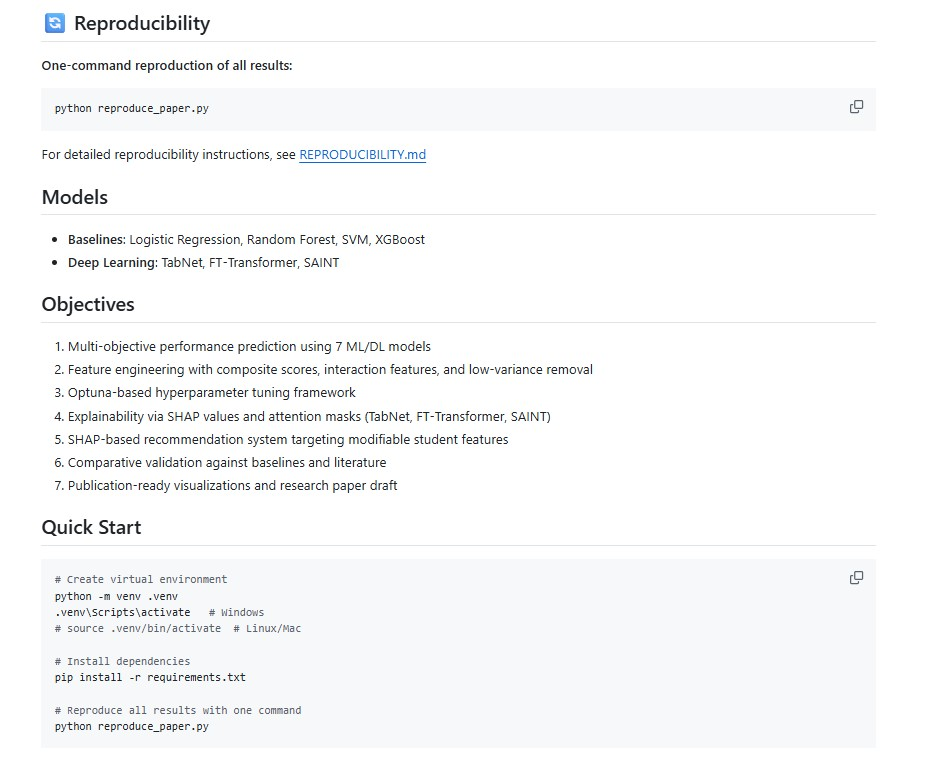
\includegraphics[width=\textwidth]{I1.jpg}

\vspace{6pt}

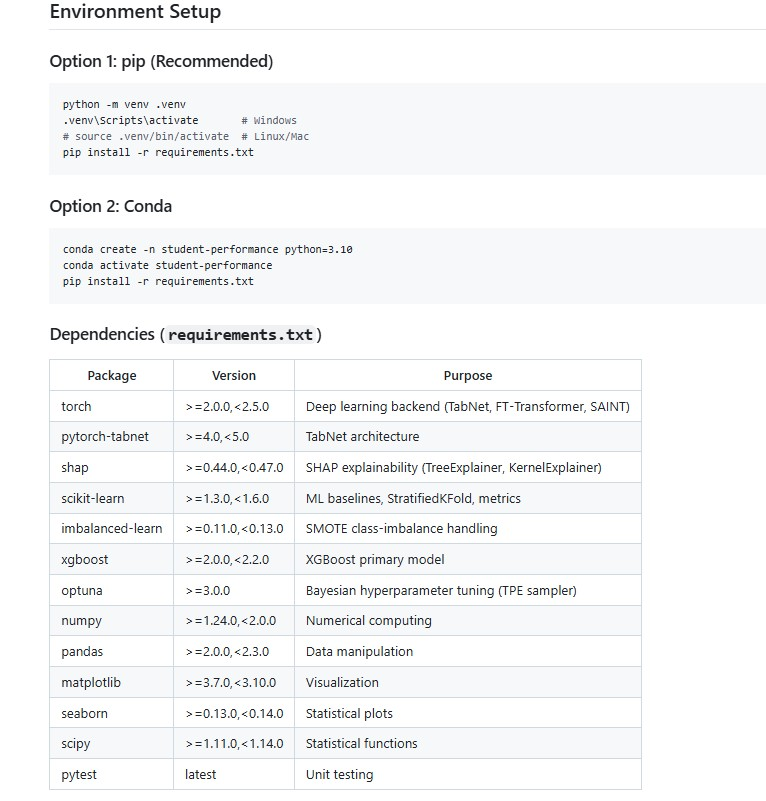
\includegraphics[width=\textwidth]{I2.jpg}

\vspace{6pt}

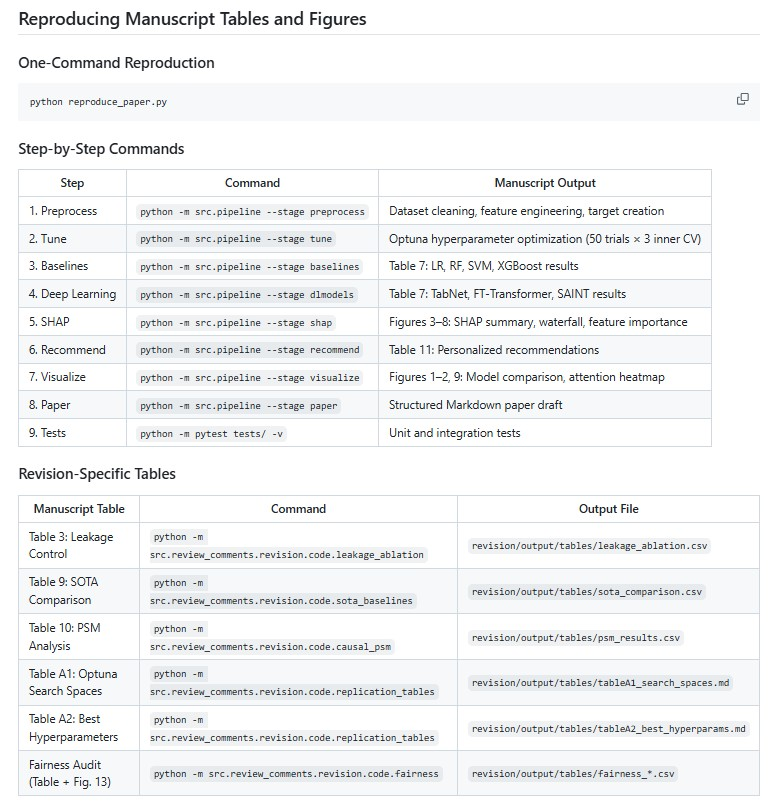
\includegraphics[width=\textwidth]{I3.jpg}

\vspace{6pt}

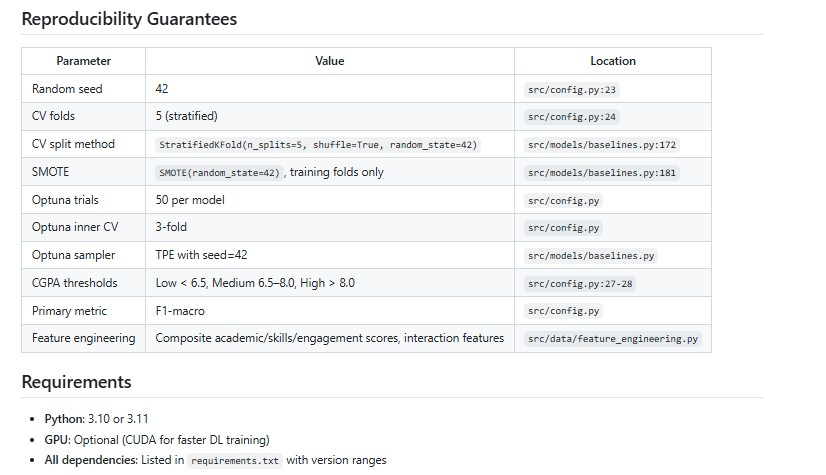
\includegraphics[width=\textwidth]{I4.jpg}

\vspace{6pt}

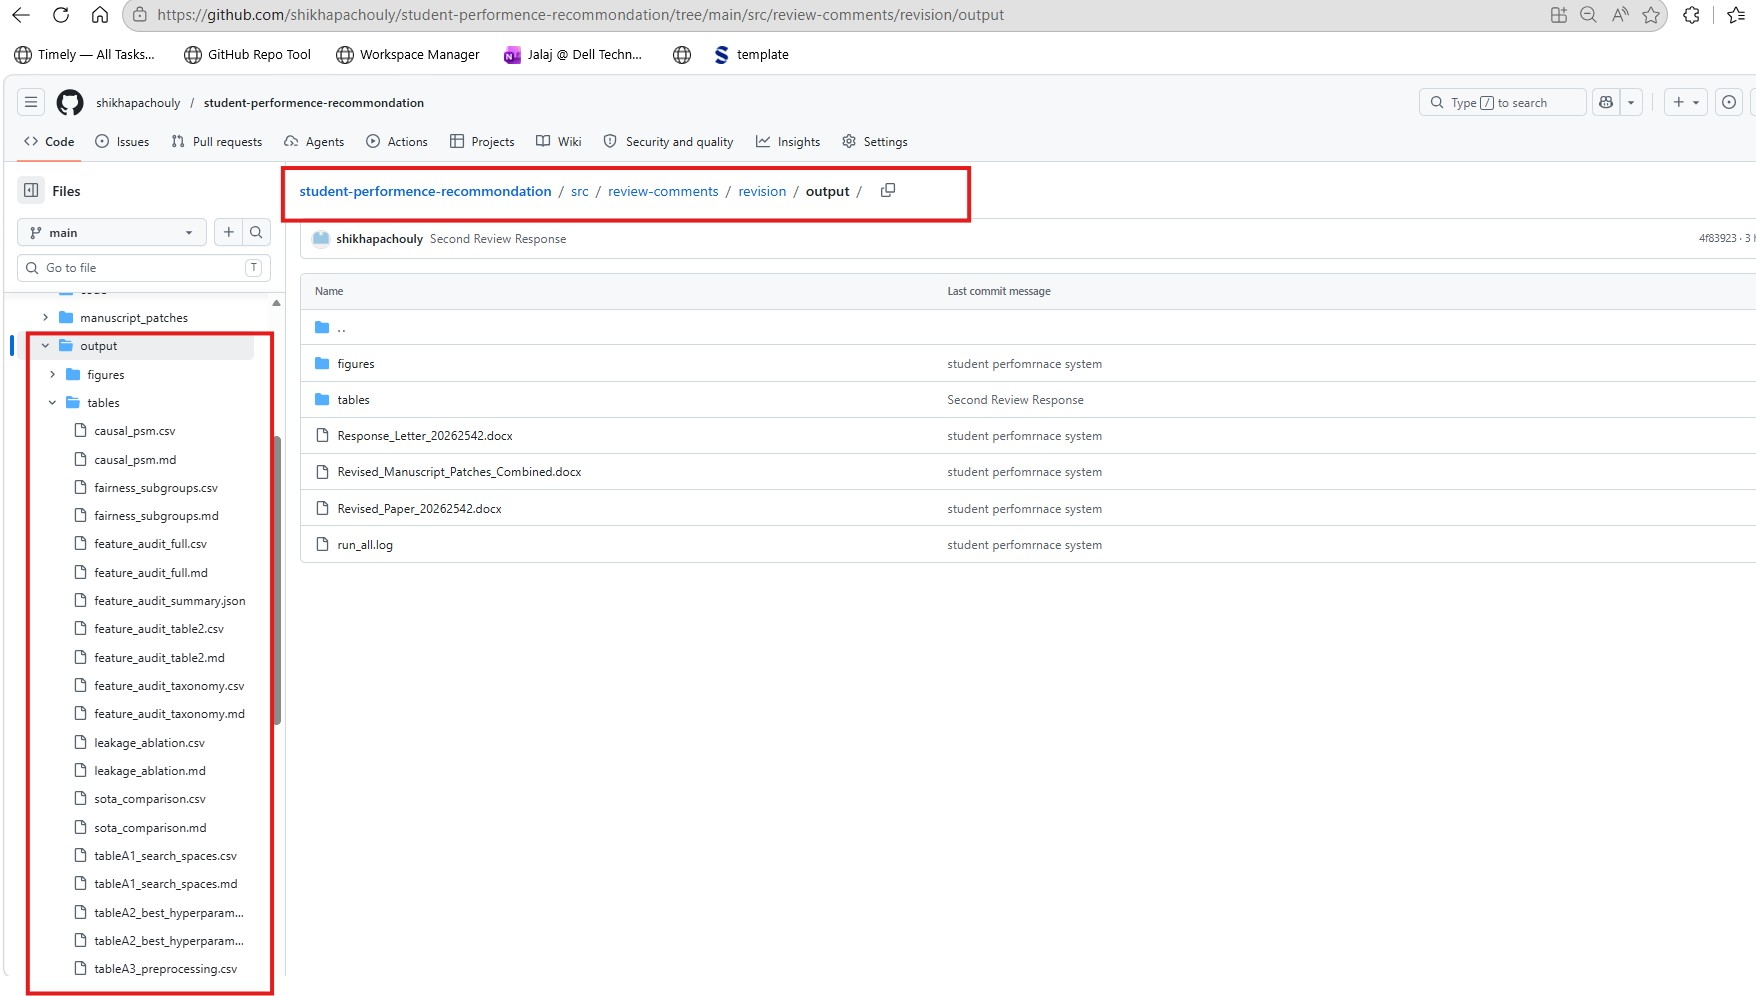
\includegraphics[width=\textwidth]{I5.jpg}
\end{center}



\begin{correctionbox}
\noindent \textbf{Response summary:} The GitHub repository \stress{ contains ALL mandatory reproducibility materials}:
\begin{itemize}
  \item \stress{Preprocessing \& feature engineering:} \filebox{src/data/preprocessor.py}, \filebox{src/data/feature\_engineering.py}
  \item \stress{Fold indices:} Deterministic via \texttt{StratifiedKFold(seed=42)}, identical every run
  \item \stress{Optuna search spaces:} \filebox{src/config.py:352--430} for all 7 models
  \item \stress{Best hyperparameters:} Logged during training; Table~A2 via revision code
  \item \stress{SMOTE:} \texttt{SMOTE(random\_state=42)}, training folds only
  \item \stress{Random seeds:} \texttt{RANDOM\_SEED = 42} in \filebox{src/config.py:23}
  \item \stress{Environment:} \filebox{requirements.txt} with version-pinned dependencies
  \item \stress{Instructions:} \filebox{README.md} with explicit command tables for every table and figure; \filebox{REPRODUCIBILITY.md} for detailed guide
  \item \stress{Dataset:} \filebox{dataset/student-dataset.csv} (anonymized, 597KB)
\end{itemize}

\end{correctionbox}

% =============================================================================
% ADD NEW COMMENTS ABOVE THIS LINE
% =============================================================================

\vspace{12pt}
\hrule
\vspace{6pt}

\section*{Summary of Corrections}

\begin{center}
\begin{tabular}{l l p{8cm}}
\toprule
\textbf{ID} & \textbf{Type} & \textbf{Description} \\
\midrule
\cid{CORR-1} & Numerical error & Table 2 delta for CGPA Category corrected from 0.063 to 0.064 \\
\cid{CORR-2} & Methodological clarification & Table 9: Explicitly stated that workshop participation recommendation is predictive-only (SHAP = 0.331) and not supported by causal evidence due to n matched = 0 in PSM analysis \\
\cid{CORR-3} & Clarification needed & Student count and CGPA distribution: Percentages are rounded (8.1\%/56.2\%/35.6\%); actual counts are Low: 112 (8.13\%), Medium: 775 (56.24\%), High: 491 (35.63\%), sum = 1,378. Will update distribution table to include both counts and percentages \\
\cid{CORR-4} &  Addressed & Optuna search budget is normalized by trials (50 $\times$ 3 = 150 evaluations per model). Search-space dimensionalities are comparable (4--5 params each). \sectref{4.3}  states gap ``cannot be attributed to under-tuning'' and frames DL underperformance as regime-specific. No changes needed \\
\cid{CORR-5} & Addressed & SOTA comparison fairness: All baselines use identical CV splits (seed=42), identical 48-feature matrix, identical leakage prevention (7 columns dropped, SMOTE on train only), and identical F1-macro metric. Gap attributed to engineered features, not unfair conditions. \sectref{5.4} states this. \\
\cid{CORR-6} & Completed & GitHub reproducibility: Git repository contains all required artifacts. Deterministic seed=42 ensures reproducible folds. Optuna spaces in config.py:352-430. Best params logged during training. Dataset included (597KB). Revision code reproduces all tables. Complete instructions in multiple READMEs. No changes needed \\
\midrule
% Add new corrections to this summary table
\bottomrule
\end{tabular}
\end{center}

\vspace{6pt}
\hrule
\vspace{6pt}

\noindent \textit{Last updated: May 23, 2026}

\end{document}
